This thesis aims to improve medical imaging and pre-operational planning by using a modern approach with head-mounted displays.
By using acquired 3D medical imaging in a virtual reality application, a very patient specific, highly realistic and only moderately costly technique with which surgeons can prepare for operations is pursued.

This thesis aims to achieve the following advantages over conventional methods:
\begin{compactenum}[label=(\alph*)]
    \item Familiarize the operator with the patient specific anatomy and pathalogy before operating
    \item The ability to simulate important operation steps
    \item Allow revision of the virtual operation as often as needed
    \item Recording and analysis of users and others virtual operations
    \item Test out procedures
\end{compactenum}

Especially the imaging of voluminous objects is mentally demanding and this thesis hopes to eliminate this problem completely by providing realistic 3D medical imaging in virtual reality.
This thesis is part of an applied virtual and augmented reality workflow for oral and maxillofacial surgery using head mounted displays (HMDs) as described in Figure \ref{fig::ProjectPlan}.

\begin{figure}[ht!]
    \centering
    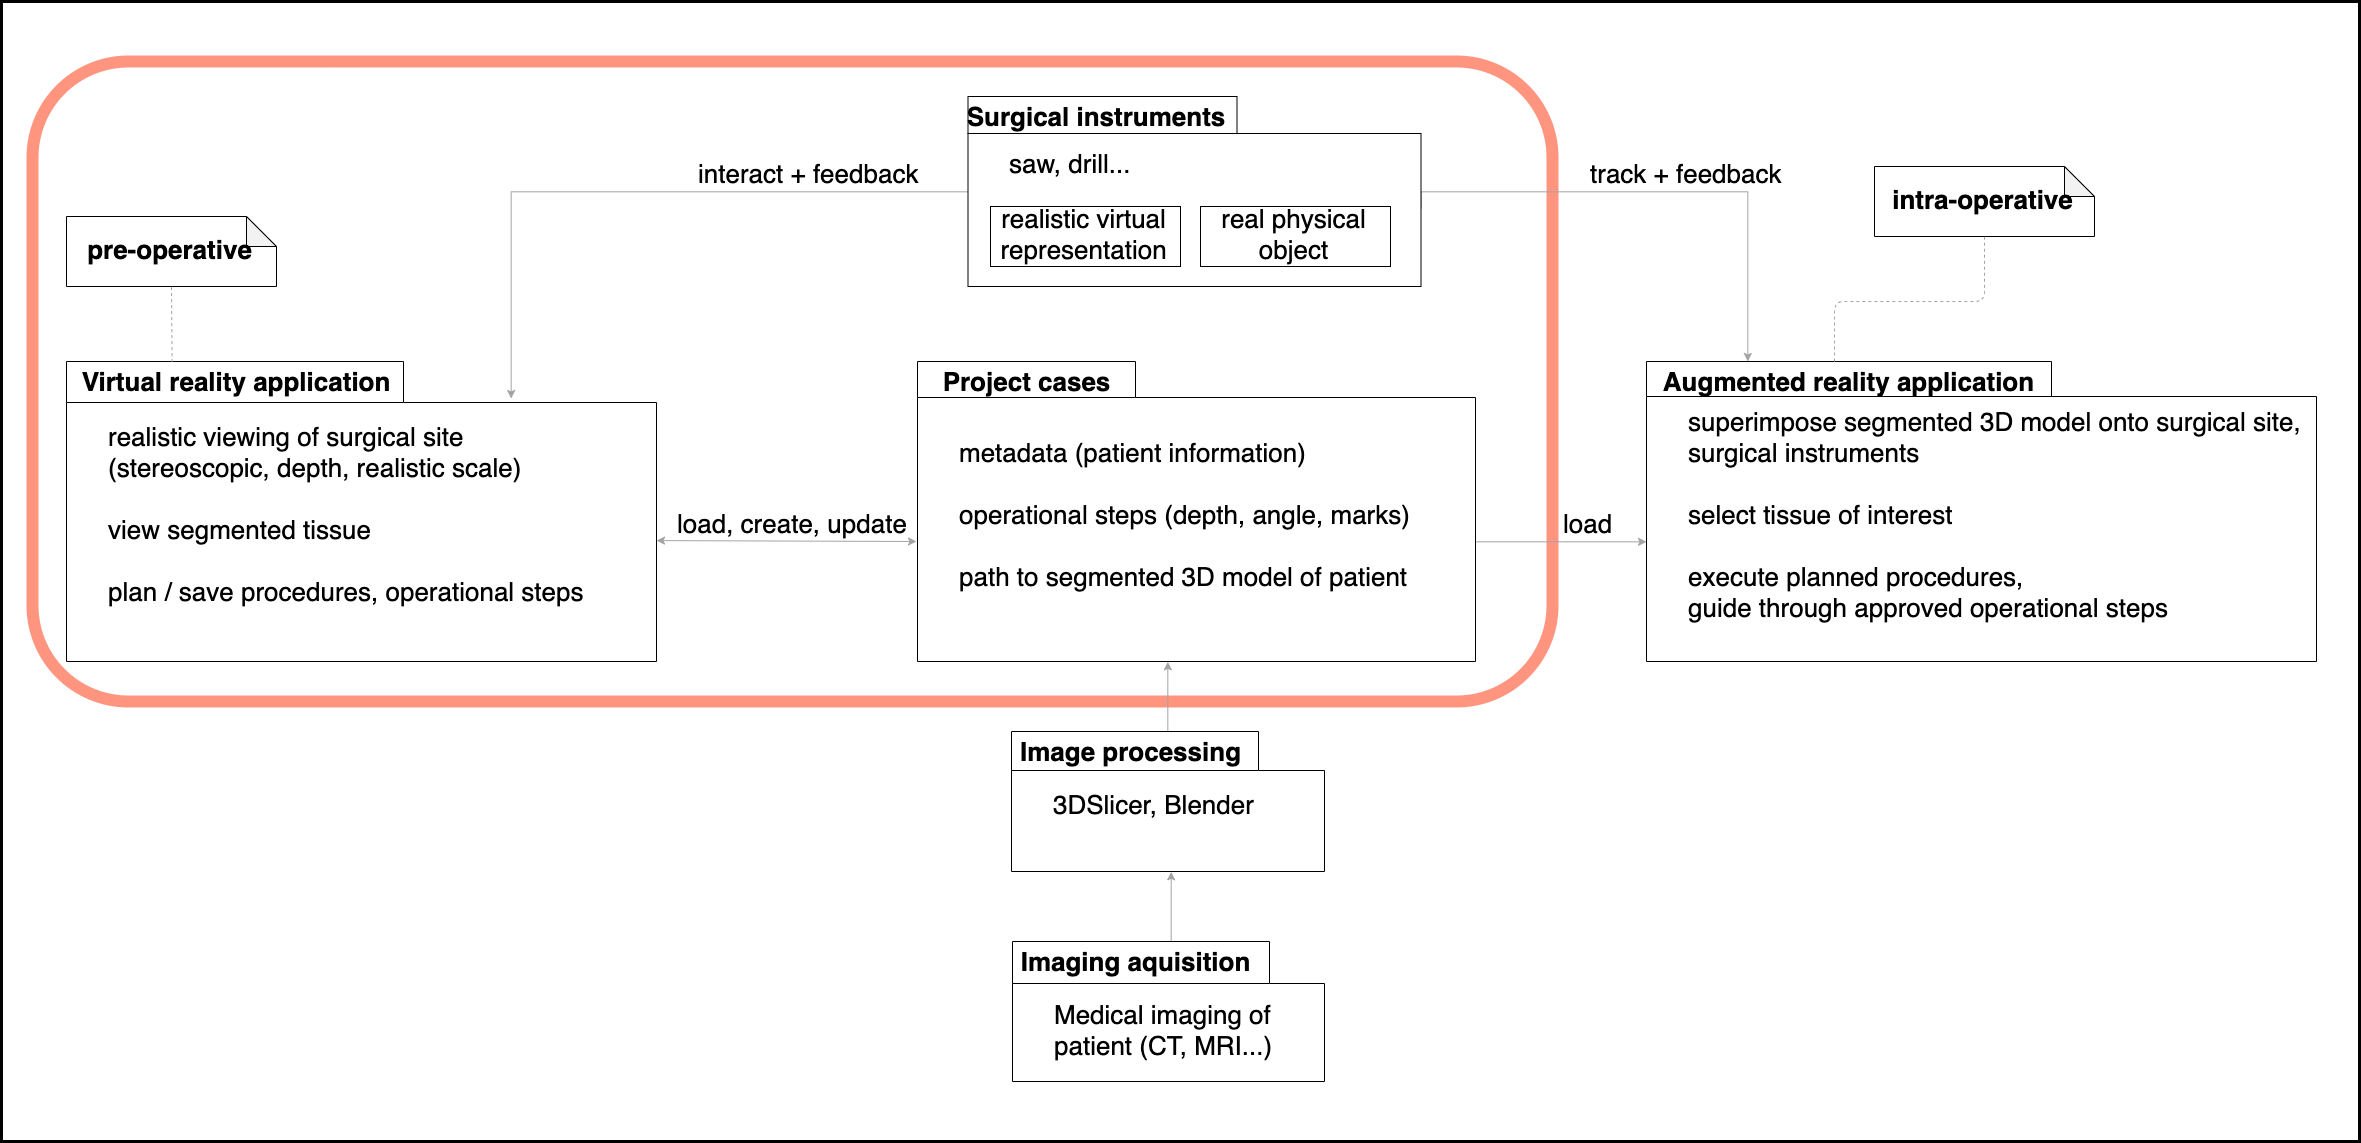
\includegraphics[width=\linewidth]{images/project_plan.png}
    \caption{\label{fig::ProjectPlan} Complete VR and AR workflow for surgeons concept}
\end{figure}

The main goal of this thesis is to create a pre-operative assistance tool in VR with HMDs for oral and maxillofacial surgery as highlighted in Figure \ref{fig::ProjectPlan}. 
In addition, the results of the pre-operative planning might be used intra-operatively to provide assistance via Augmented Reality (AR) as described in the workflow.
To provide a useful preparational tool, it is critical to simulate individual operation steps.
Planned steps will be storable in a format in which they can be loaded and viewed in both the virtual and augmented reality applications bi-directionally as described.
By planning the operational steps in virtual reality, planned procedures can easily be shown to other staff involved.
Naturally, it will be of uttermost importance that we have medical equipment and an appropriate virtual environment recreated remarkably close to reality.

The remainder of this Thesis is structured as follows: TODO